\subsection{$d(K^-, p)"\pi^-\Sigma^0"$ and $d(K^-, p)"\pi^-\Lambda"$ cross section}
\input{analysis/KP_scaling_table} % To do 票の並びを変える
We obtained spectra identified final state of the $d(K^-, p)"\pi^-\Lambda"$ and the $d(K^-, p)"\pi^-\Sigma^0"$.
These spectra were corrected the solid angle due to the bending angle by the Ushiwaka and the acceptance of the CDS.
After that, spectra were converted to the differential cross section ($\frac{d^2\sigma}{d\Omega dm}$) using the luminosity and detector efficiencies.
The first one is luminosity which was consists of the number of target, the number of irradiated kaon, the DAQ live rate, and the trigger efficeincy.
The number of target was defined from the length of fiducial volume ($10cm$) and target density which was evaluated from measured temperature which was described in Sec\ref{sec:target}.
The number of irradiated kaon was defined by correcting kaon number counted up by the scaler DAQ by the ratio of true kaon in kaon trigger which was described in Sec\ref{sec:beam_line_ana}.
About DAQ live rate and trigger efficiency were described in Sec\ref{sec:trigger}.

Next is about detector efficiencies.
There were detector efficiencies of the CDS and forward detectors which were described Sec\ref{sec:CDC_eff} and Sec\ref{sec:FC_eff}.
The CDC efficiency was due to the inefficient event of the chamber.
The analysis efficiency was convoluted to the acceptance which was estimated using the MC sim with the same analysis procedure of the data analysis.
The forward efficiency included the analysis efficiency and the reaction loss and so on because the efficiency was estimated using the missing proton from the $d(K^-, \Lambda \pi^-)"p"$ reaction.

These parameters were summarized to Table\ref{tab:KP_scale},
in which the survival ratio of $K^-$, the DAQ live ratio and the trigger efficiency were represented typical value although these were estimated run-by-run.

We obtained the cross sections of the $d(K^-, p)"\pi^-\Lambda"$ and the $d(K^-, p)"\pi^-\Sigma^0$ to adopt these correction and scaling, which were represented in Fig\ref{fig:pimL_CS} and Fig\ref{fig:pimS0_CS}.
In these plots, boxes indicate independent errors on bins which were caused by statistic error, the solid angle estimation, and the acceptance estimation
and error bars indicate commonly error each bin which  was caused by conversion factor.

\begin{figure}[htbp]
  \centering
  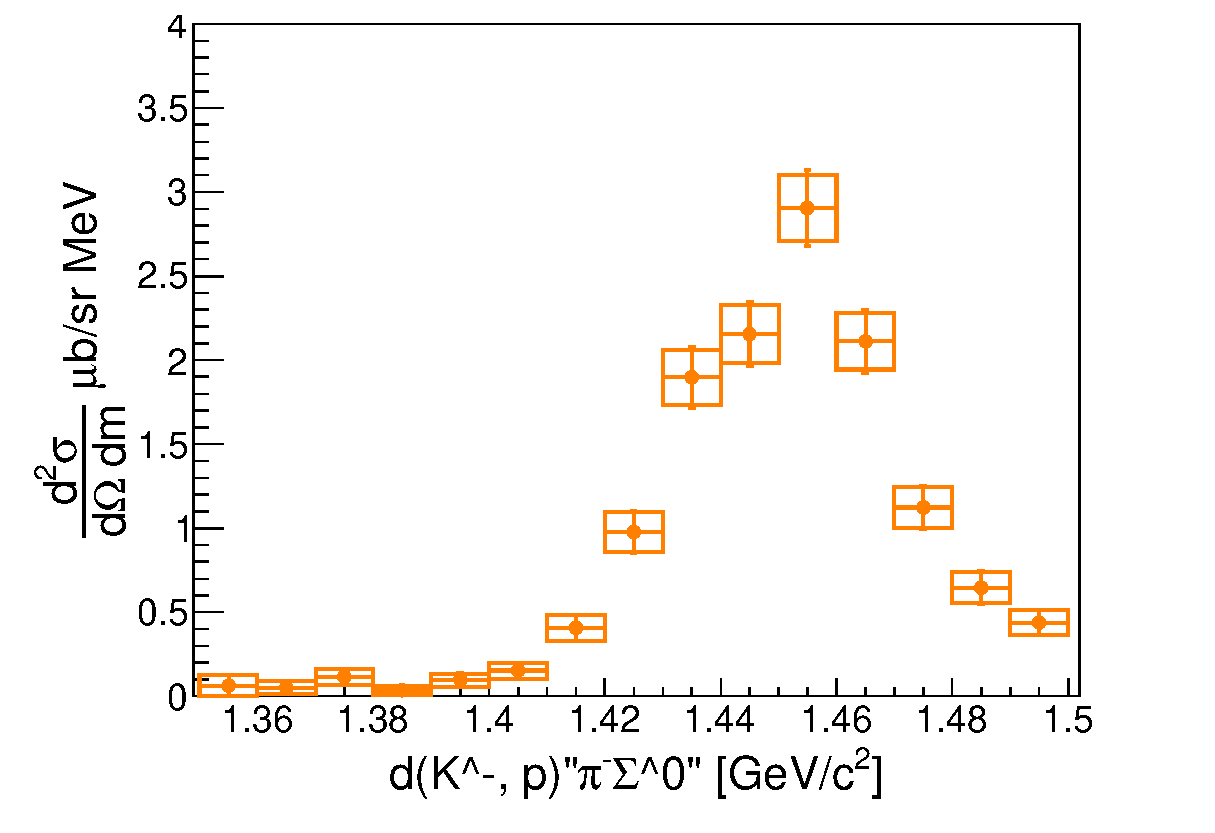
\includegraphics[width=10cm]{../pic/Run68/KP_ana/pimS0_CS_zoom.eps}
  \caption{
    The cross section of $d(K^-, p)"\pi^-\Sigma^0$ mode.
  }
  \label{fig:pimS0_CS}
\end{figure}

\begin{figure}[htbp]
  \centering
  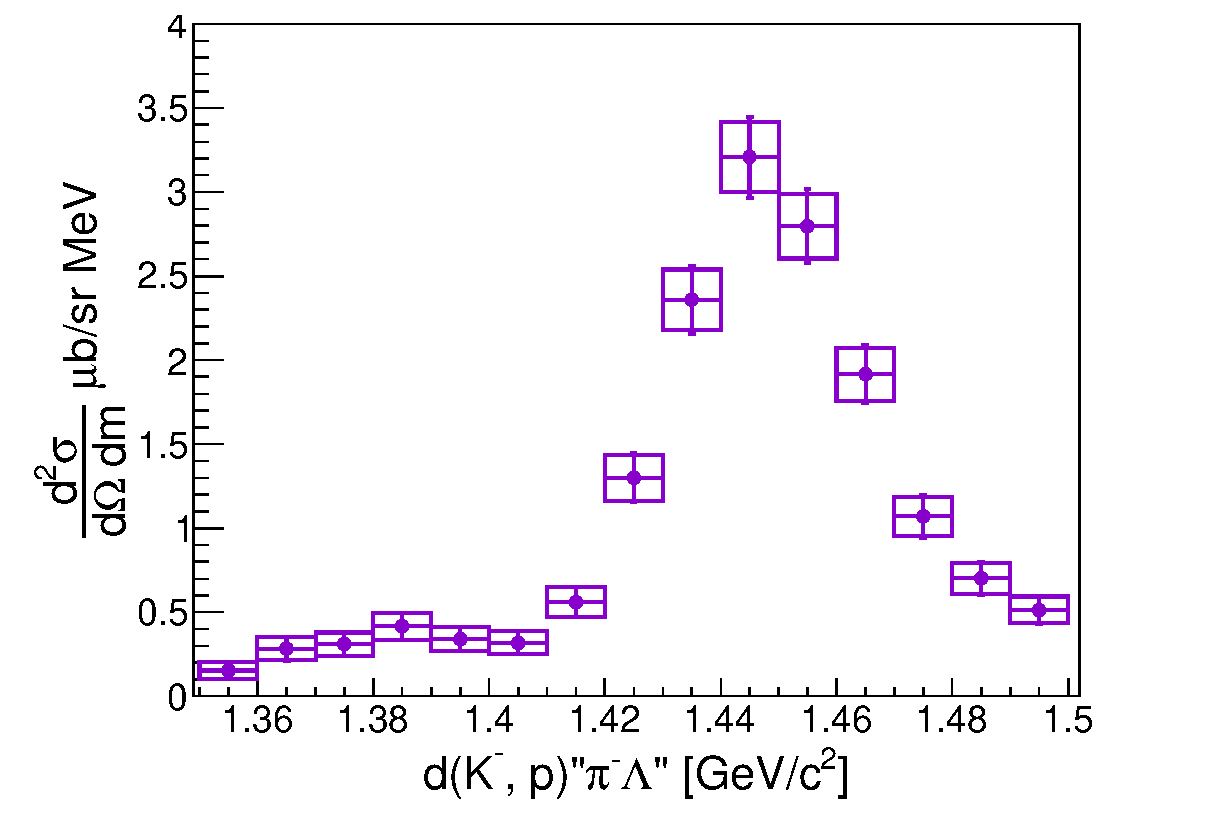
\includegraphics[width=10cm]{../pic/Run68/KP_ana/pimL_CS_zoom.eps}
  \caption{
    The cross section of $d(K^-, p)"\pi^-\Lambda^0$ mode.
  }
  \label{fig:pimL_CS}
\end{figure}


